\chapter{Wykład 9. Zarządzanie czasem w projekcie informatycznym}

\section{SPP uwzglęniający plan kont kosztowych projektu}
% strona 34

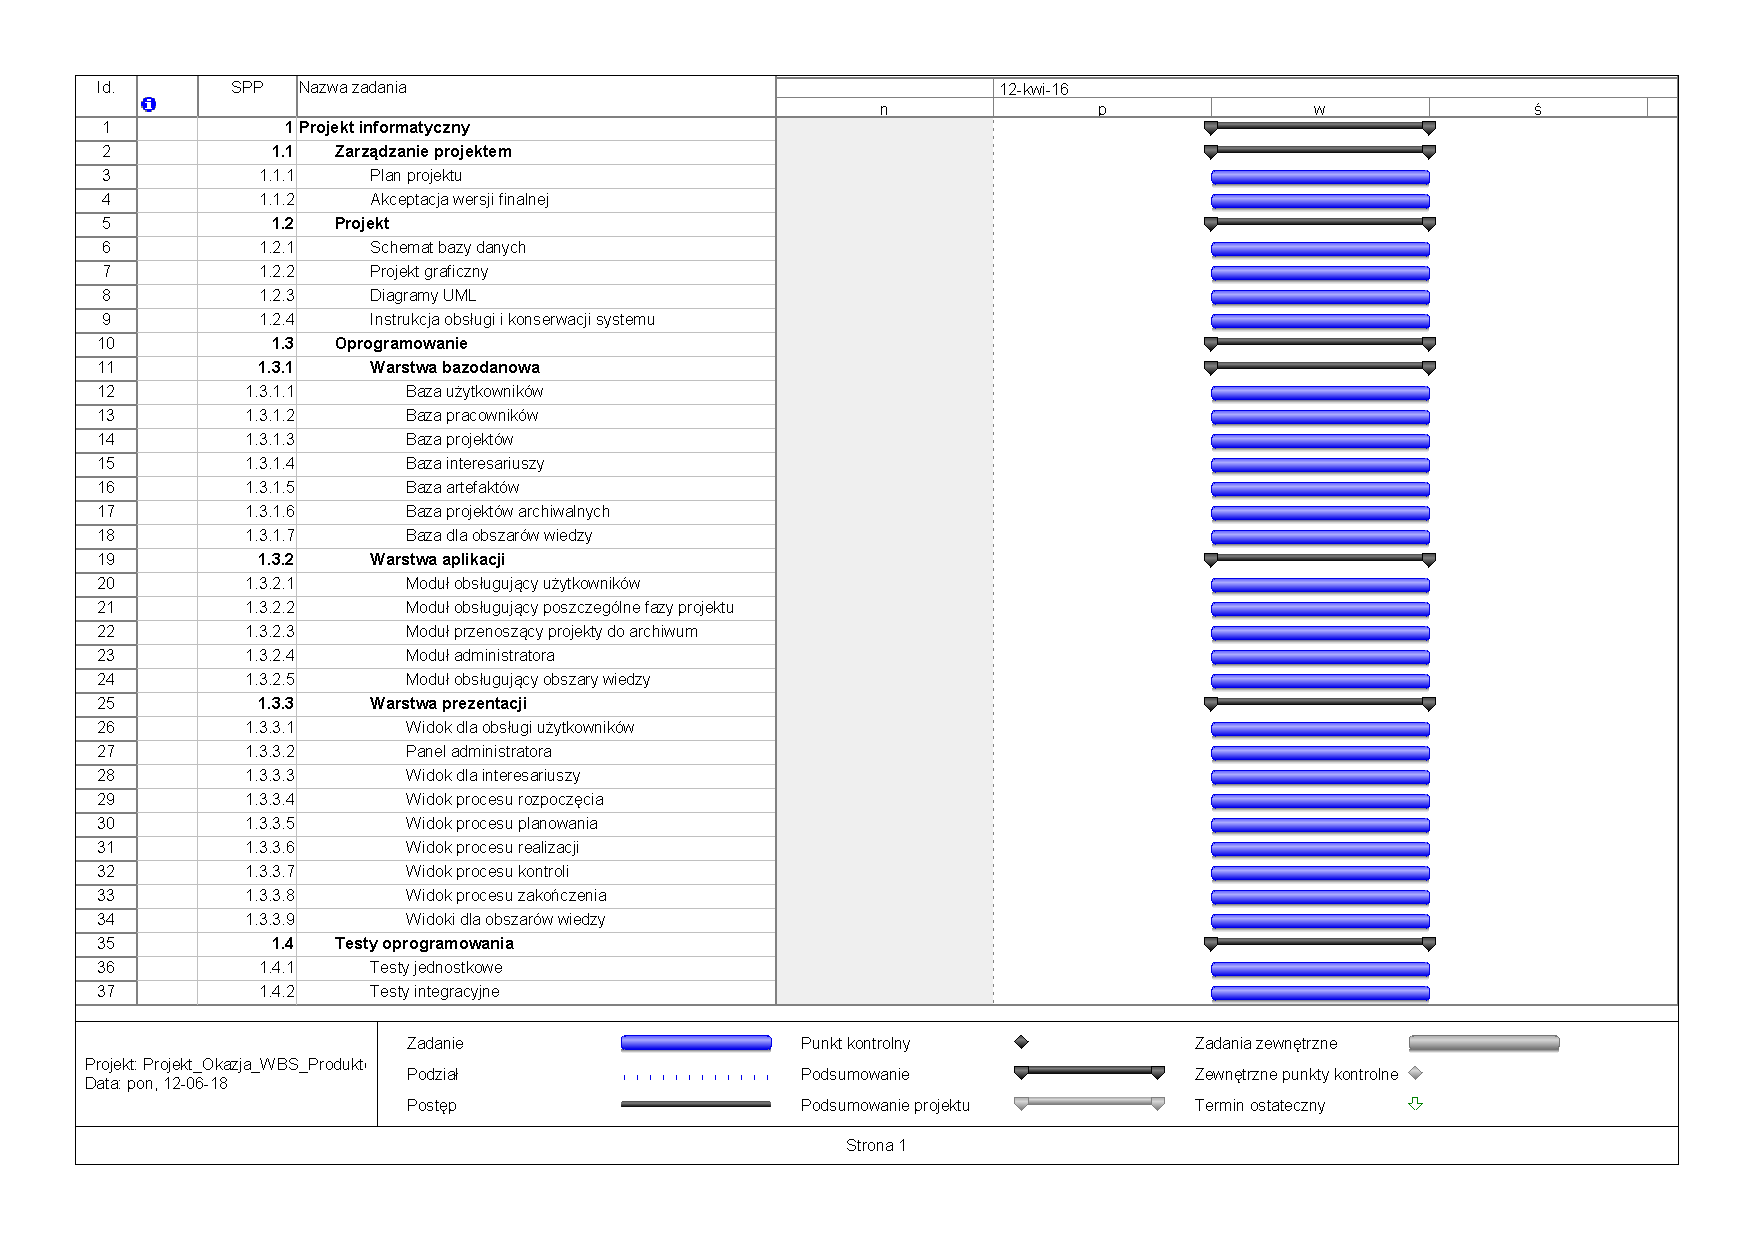
\includepdf[nup=1x2,pages=-]{diagramSPP.pdf}

% ===========================================================================

\section{Harmonogram w MS Project}
% strona 35

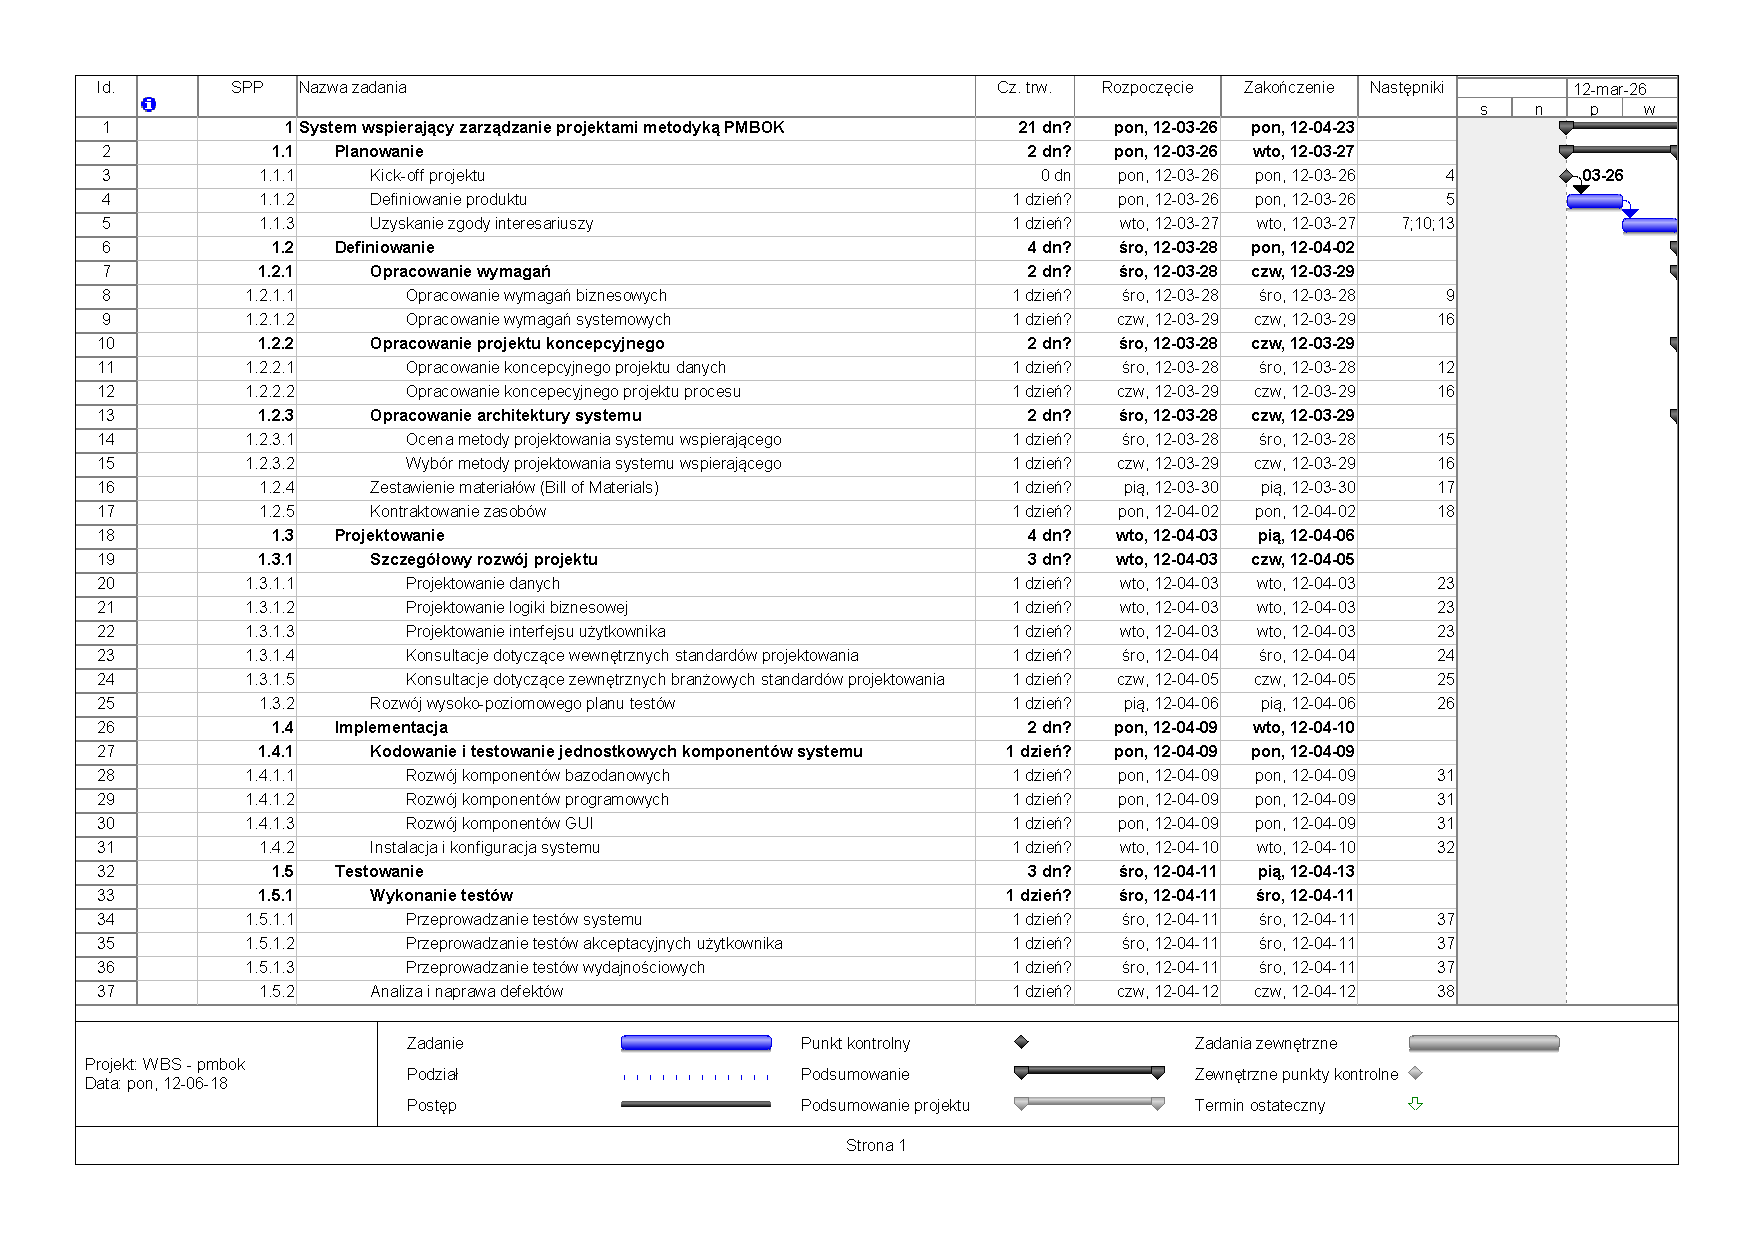
\includepdf[nup=2x2,pages=-,landscape=true,column=true]{harmonogramWBS.pdf}

% ===========================================================================

\begin{landscape}

\section{Struktura RBS projektu}
% strona 45

\begin{figure}[!h]
\centering
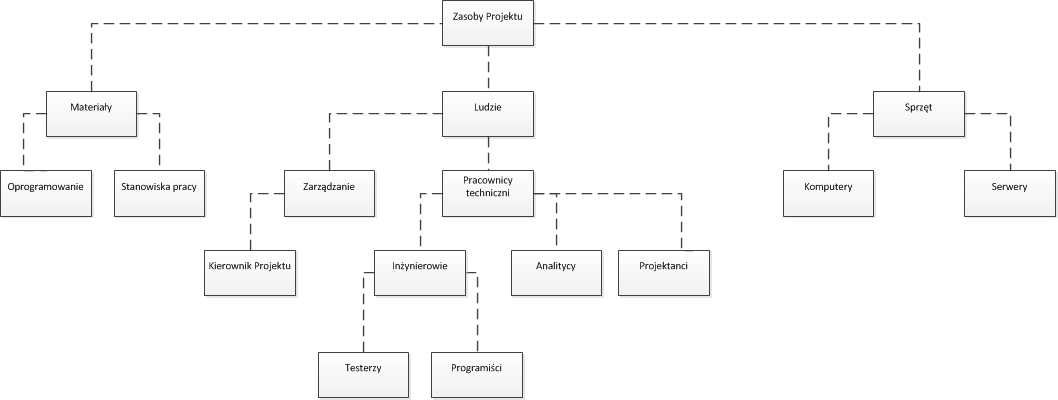
\includegraphics[width=1.5\textwidth]{RBS.png}
\caption[RBS]{RBS}
\label{rysunekProces}
\end{figure}

\end{landscape}
% ===========================================================================

\section{Zasada szacowania działań}
% strona 52
Nasza firma jest przedsiębiorstwem z wieloletnim doświadczeniem zdobytym przy realizacji licznych projektów o zróżnicowanej tematyce. Uznaliśmy, że warto wykorzystać to doświadczenie przy kolejnych projektach, dlatego zasadę szacowania czasów trwania działania opieramy o metodę szacowania przez analogię. Szacowaniu podlegają elementy z najniższego (najbardziej podstawowego) poziomu WBS, a szacującym jest zazwyczaj osoba odpowiedzialna za realizację danego elementu w oparciu o dokumentację z poprzednich projektów. 

	Przykład.\\
Konieczne jest oszacowanie czasu wykonania projektu interfejsu użytkownika naszej aplikacji. Dotychczas nasza firma wykonywała już 2 podobne, choć nie aż tak skomplikowane, szkice. Poprzednie projekty zajęły po pół dnia. Ponieważ aktualny interfejs będzie bardziej złożony od dotychczas realizowanych, przewidujemy, że jego zaprojektowanie zajmie 1 dzień.

% ===========================================================================


\section{Harmonogram z uwzględnieniem zasobów}
% strona 59

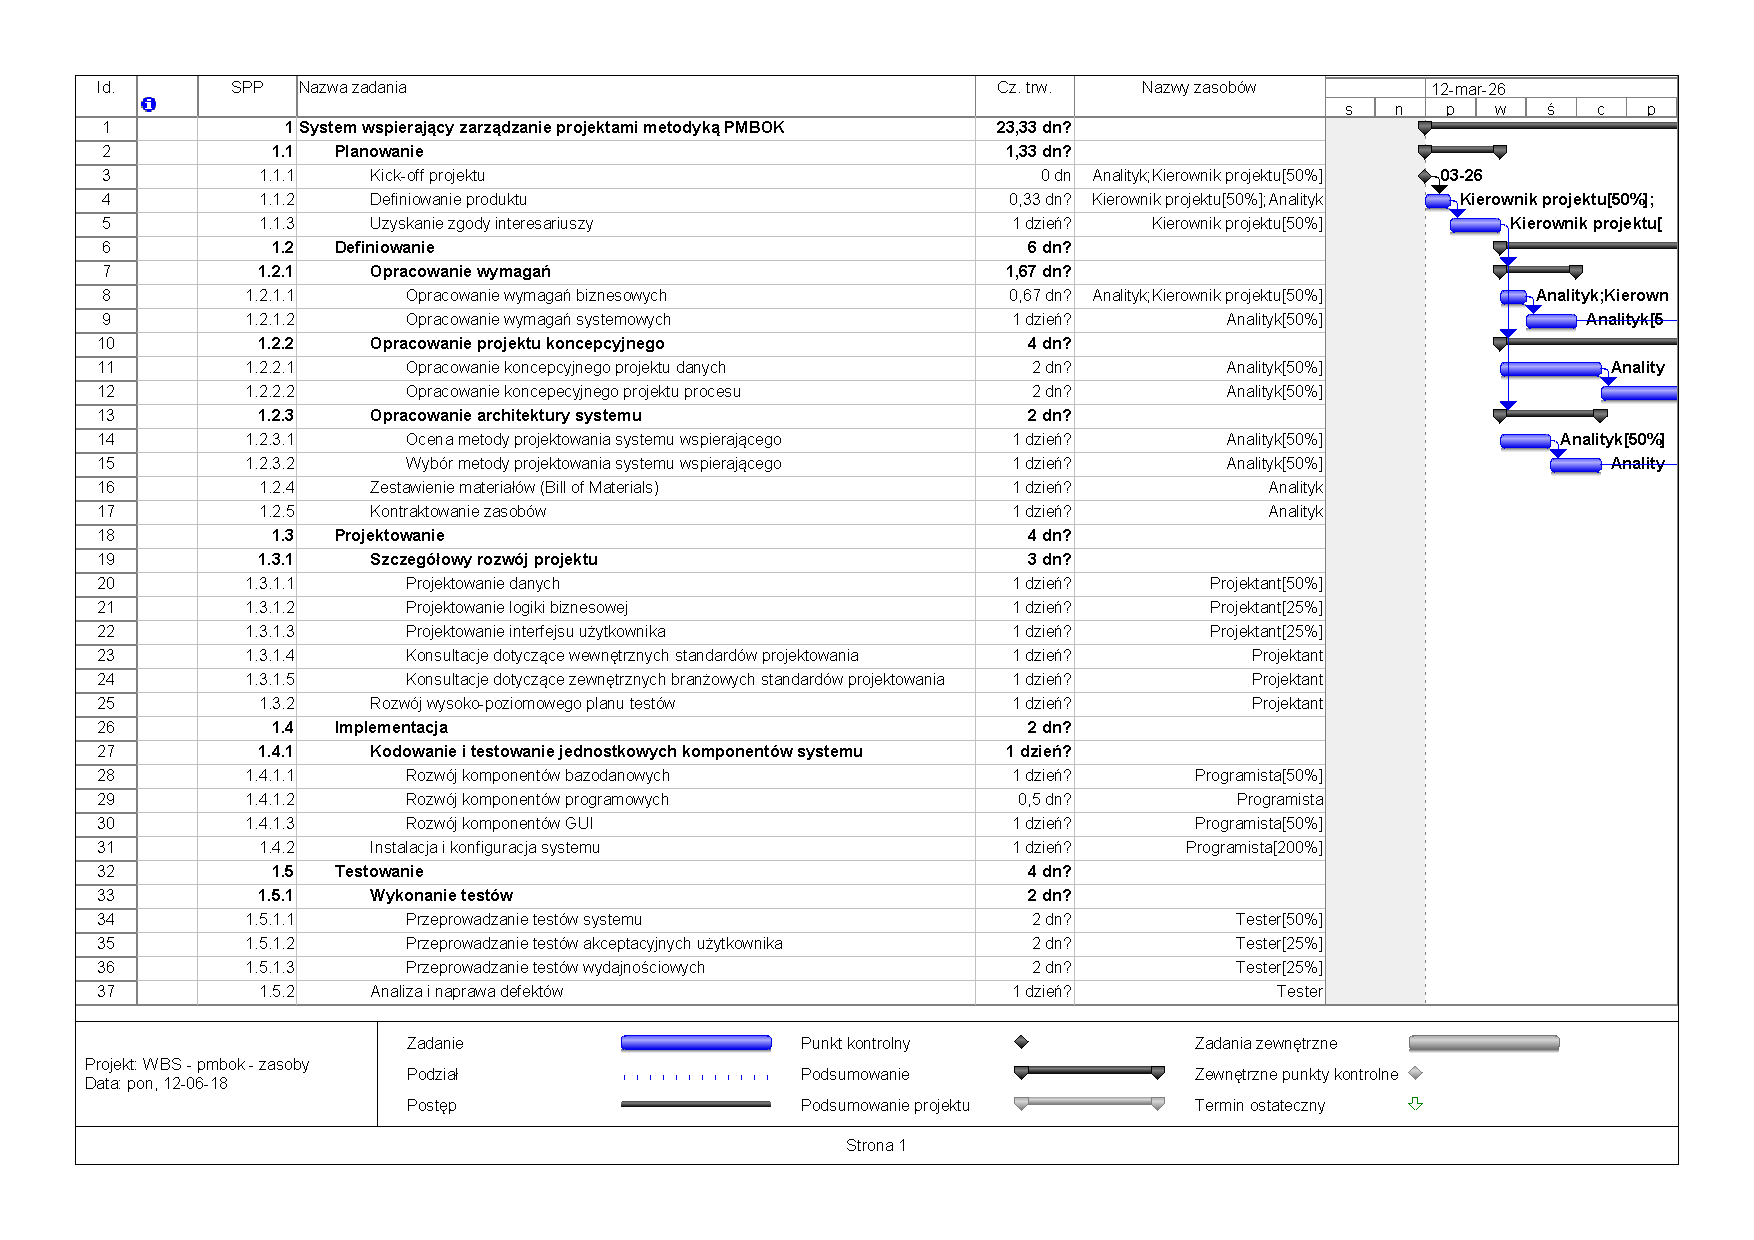
\includepdf[nup=2x2,pages=-,landscape=true,column=true]{zasobyWBS.pdf}

